
%%%%%%%%%%%%%%% Team Intro Page %%%%%%%%%%%%%%%%%%%%
\clearpage
\section{Team Structure}
\subsection{Team Member 1}
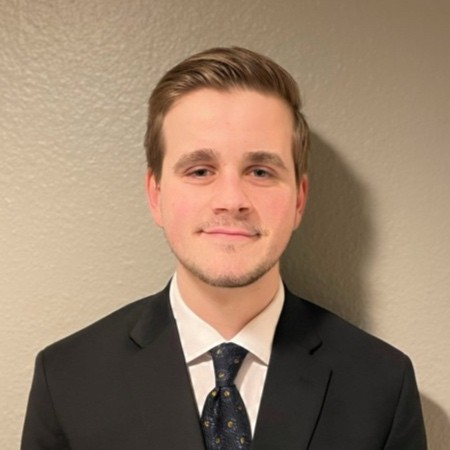
\includegraphics[height=4cm]{images/david.jpg} \\
\textbf{David Thoe}\\
Major: Electrical Engineering\\
Contact: dthoe@purdue.edu\\
Team Role: Team Leader \\
Bio: In charge of graphics drivers and text display, I will be focused on the final presentation of the information as well as subsystem integration.
I will also be paying special attention to the housing of the prototype, aided by CAD and 3D printing, ensuring the product appears polished when complete.
At Purdue, I concentrate in Wireless and Optical engineering and participate in the club Autonomous Motorsports Purdue, where we place our fully autonomous go-kart in competition with other univiersities.
In my free time, I work on hobby electrical projects usually related to my computer or decoration.

\subsection{Team Member 2}
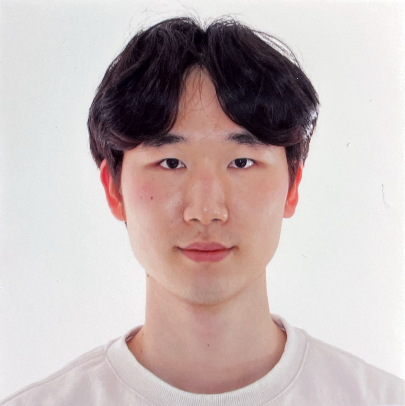
\includegraphics[height=4cm]{images/joshua.png} \\
\textbf{Joshua Kim}\\
Major: Electrical Engineering\\
Contact: kim3503@purdue.edu\\
Team Role: Communication Lead \\
Bio: In my role as Communication Lead,
I am responsible for ensuring that communication on our
team, with GTA, and the Professor is clear and consistent.
I manage communications on updates, facilitate collaboration on
progress reporting, and keep everyone engaged and aligned within
the subsystem groups to further our design as a cohesive project.
My background in Electrical Engineering enables me to contribute
directly to the technical aspects of the project and also help
translate technical details into clear explanations for our team
and other stakeholders. Balancing the communication and development
of the subsystem, I can keep both the engineering work and project
coordination rolling smoothly.

\subsection{Team Member 3}

\includegraphics[height=4cm]{images/zeke.png} \\
\textbf{Zeke Ulrich}\\
Major: Computer Engineering\\
Contact: pulrich@purdue.edu\\
Team Role: Treasurer \\
Bio: Zeke is the processing and PCB design specialist.
He's responsible for designing the PCB schematics and
integrating the disparate subsystems on the processor.
At Purdue, Zeke belongs to the Marine Corp Officer Candidate Program,
Eta Kappa Nu, Tau Beta Pi, and Purdue's Effective Altruism community.
Outside Purdue, he is president of the nonprofit DuelGood and works
for the government in cybersecurity.
In the future he hopes to study international relations as a Truman
scholar, start a family, and volunteer as a firefighter.
He enjoys athletics and spending time with his friends.

\subsection{Team Member 4}
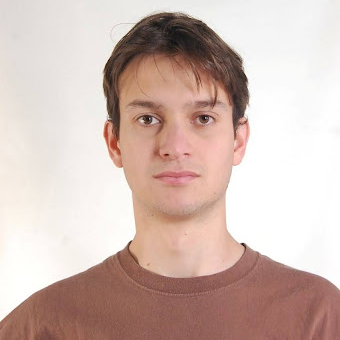
\includegraphics[height=4cm]{images/juan.png} \\
\textbf{Juan Vargas}\\
Major: Electrical Engineering\\
Contact: varga105@purdue.edu\\
Team Role: Facilitator \\
Bio: As the Facilitator, my primary role is to keep our team
organized, collaborative, and on track throughout the project.
I focus on making sure discussions are productive, tasks are
clearly divided, and deadlines are met without overwhelming
any single member. By bridging technical conversations and
helping resolve roadblocks quickly, I ensure that progress
stays steady and balanced across subsystems. Alongside this
coordination, I contribute to the technical development by
assisting with software and system integration specially in
the network/communication part, ensuring our device works as
intended while maintaining the retro, aviation-inspired feel
that defines Aviator.